\section*{Abstract}
The Ywing is a VTOL (vertical take off and landing) drone capable of flying at any speed between its cruise speed and hover by varying its angle of attack. The angle of attack (angle between wing chord and airflow) cannot always be approximated by pitch angle (angle between wing chord and horizon) because the drone is not always flying at constant altitude or undergoes some wind. The goal of this project is to use optic flow measurements from a wide field of view camera embedded on the drone to estimate the angle of attack. Indeed, in translation flight, all optic flow vectors point to the current direction of flight, which can be used to estimate angle of attack. The estimation of angle of attack will be implemented on the onboard controller using optic flow vectors computed on the camera, and validated in flight. If time allows, this estimate will be used to control the altitude of the Ywing.

\section{Introduction}

\section{Theoretical background}	

\subsection{Omnidirectional Camera Model}
An omnidirectional camera provides wide field of view, at least 180 degrees. In our case, we used a dioptric camera, which uses a combination of shaped lenses (fisheye lenses) and typically can reach a field of view slightly larger than 180 degrees. 

A wide field-of-view is preferred for optic-flow-based egomotion estimation because it is necessary to distinguish clearly the direction of motion out of multiple optic-flow measurement. It also allows for more robustness and redundancy in a variety of environments and conditions.

All modern fisheye cameras are central, and hence, they satisfy the single effective focal point property. The reason a single effective viewpoint is so desirable is that it allows us to generate geometrically correct perspective images from the pictures captured by the omnidirectional camera. When the geometry of the omnidirectional camera is known, that is, when the camera is calibrated, one can precompute this direction for each pixel. Therefore, each pixel can be mapped onto a plane at any distance from the viewpoint to form a planar perspective image. Additionally, the image can be mapped onto a sphere centered on the single viewpoint, that is, spherical projection.

Omnidirectional camera systems cannot be described using conventional pinhole model because of the very high distortion induced by the imaging device. Indeed, in our case, the model should take into account the refraction caused by the lens of the fisheye camera. A unified model was proposed in \cite{scara}. To overcome the lack of knowledge of a parametric model for fisheye cameras, a Taylor polynomial, whose coefficients and degree are found through the calibration process, is used.

Let $p$ be a pixel point of your image, and $(u,v)$ its pixel coordinates with respect to the center of the omnidirectional image. Let $P$ be its corresponding 3D vector emanating from the single effective viewpoint, and $(x,y,z)$ its coordinates with respect to the axis origin. The function estimated by the calibration process maps an image point $p$ into its corresponding 3D vector $P$:\\
\begin{equation}
\label{equ:cameraModel1}
P = \begin{bmatrix}
		x\\
		y\\
		z\\
	\end{bmatrix}
	= \begin{bmatrix}
		u\\
		v\\
		f(r)\\
	  \end{bmatrix}
\end{equation}
where 
$
\begin{cases}
r = \sqrt{u^2 + v^2}\\
f(r)= a_0 + a_1r + a_2r^2 + a_3r^3 + a_4r^4 + ...\\
\end{cases}
$\\
and the parameters to estimate are $a_0$, $a_1$, $a_2$, ...
Although increasing the polynomial may yield better accuracy, we used 4\textsuperscript{th} order polynomials, as a good trade-off between accuracy and complexity of the polynomial model.

However, as the camera and mirror axes are never perfectly aligned, the model is extended so as to model these errors through an affine transformation:
\begin{equation}
\label{equ:cameraModel2}
\begin{bmatrix}
u'\\
v'\\
\end{bmatrix}
=
\begin{bmatrix}
c & d\\
e & 1\\
\end{bmatrix}
\cdot
\begin{bmatrix}
u\\
v\\
\end{bmatrix}
+
\begin{bmatrix}
x_c\\
y_c\\
\end{bmatrix}
\end{equation}
which relates the real distorted coordinates $(u', v')$ to the ideal undistorted ones $(u,v)$.

This approximate model of the camera allows for more scalability in the number of optical flow measurements and more flexibility on their location, without the need to proceed to another calibration. Furthermore, the viewing directions corresponding to each pixel could be preprocessed as part of an initialization procedure to speed up subsequent computations.

The proposed calibration procedure relies on the use of a chessboard to automatically locate feature points on the camera images. Unfortunately, the resolution of our camera ($160 \times 120$) was too low for the edge detection algorithm to perform correctly its task. This issue may be avoided by using circles instead of the squares of the checkerboard. Indeed, this would yield more easily distinguishable corners. Considering this was not part of the current toolbox, we simply located 35 corners manually for each image, prior to calibration. We used 7 images taken from the camera with varying positions and orientation of the chessboard so as to cover most of the its field of view (Fig.~\ref{fig:cameraImages}). In the end, we obtained a subpixel average error of $0.34$ pixels and the following model, which relies on a 4\textsuperscript{th}-order Taylor polynomial:\\
\begin{center}
Polynomial:
$
\begin{cases}
a_0 = -6.66 . 10^{1}\\ 
a_1 = 0.00 \\
a_2 = 6.42 . 10^{-3} \\
a_3 = -2.31 . 10^{-5} \\
a_4 = 2.73 . 10^{-7} \\
\end{cases}
$
\hfill
Center:
$
\begin{cases}
x_c = 56.23 \\
y_c = 77.64 \\
\end{cases}
$
\hfill
Matrix:
$
\begin{cases}
c = 1.00 \\
d = -0.00 \\
e = -0.00 \\
\end{cases}
$
\end{center}
As we can see from the coefficients of the matrix in (\ref{equ:cameraModel2}), there is not significant misalignment between the camera and the optical lens. Hence, we can neglect this part of the model. Nevertheless, the estimated location of the center is not exactly the actual center of the $160 \times 120$ grid of pixels. The corresponding C-code implemented on the camera chip is shown in Code~\ref{code:cameraModel}.

\begin{figure}[h!]
    \centering
    \begin{subfigure}[b]{0.2\textwidth}
        \centering
        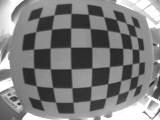
\includegraphics[width=\textwidth]{images/camera/0.png}
    \end{subfigure}
    \begin{subfigure}[b]{0.2\textwidth}
        \centering
        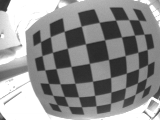
\includegraphics[width=\textwidth]{images/camera/1.png}
    \end{subfigure}
    \begin{subfigure}[b]{0.2\textwidth}
        \centering
        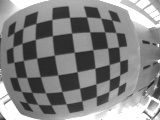
\includegraphics[width=\textwidth]{images/camera/2.png}
    \end{subfigure}
	\begin{subfigure}[b]{0.2\textwidth}
        \centering
        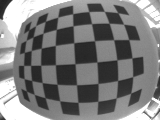
\includegraphics[width=\textwidth]{images/camera/3.png}
    \end{subfigure}
	\begin{subfigure}[b]{0.2\textwidth}
        \centering
        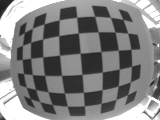
\includegraphics[width=\textwidth]{images/camera/4.png}
    \end{subfigure}
	\begin{subfigure}[b]{0.2\textwidth}
        \centering
        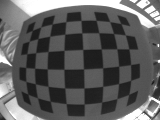
\includegraphics[width=\textwidth]{images/camera/5.png}
    \end{subfigure}
	\begin{subfigure}[b]{0.2\textwidth}
        \centering
        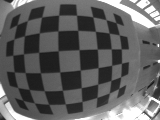
\includegraphics[width=\textwidth]{images/camera/6.png}
    \end{subfigure}
    \caption{\textbf{Training images used for camera model calibration} - The orientation and position of the chessboard were changed from one image to another to most of the field of view. The images are given in grayscale by the camera and exhibit a resolution of $160 \times 120$ pixels.}
    \label{fig:cameraImages}
\end{figure}

\begin{codeframe}[colback=white, label=code:cameraModel]{From pixels to 3D directions}
void cam2world(float *xp, float *yp, float *zp, float u, 
		float v, cam_model *cam)
{
	 float *pol    = cam->pol;
	 float xc      = cam->xc;
	 float yc      = cam->yc; 
	 float c       = cam->c;
	 float d       = cam->d;
	 float e       = cam->e;
	 uint8_t length_pol = cam->length_pol;

	 float invdet  = 1/(c-d*e);

	 // back-projection of u and v
	 *xp = invdet*(    (u - xc) - d*(v - yc) );
	 *yp = invdet*( -e*(u - xc) + c*(v - yc) );
	  
	 float r = sqrt(SQR((*xp)) + SQR((*yp)));
	 *zp  	 = pol[0];
	 
	 float r_i = 1;
	 
	 // compute z from polynomial model
	 for (uint8_t i = 1; i < length_pol; i++)
	 {
	   r_i *= r;
	   *zp += r_i*pol[i];
	 }
}
\end{codeframe}

\subsection{Mapping Optical Flow to Unit Sphere}
Now that the model of the omnidirectional camera is known - and the pixels can be mapped onto a plane or a sphere -, we can deduce the viewing direction corresponding to a given pixel. However, the particular geometry of the omnidirectional camera induces high distortions in the image. Hence, the optical flow, which is computed using Lucas-Kanade method, has to be projected onto the unit sphere using the method presented in \cite{backproj}. Mapping the optical flow directly on the unit sphere allows us to simplify further processing required for the estimation of the location of the focus of expansion, through the straightforward use of spherical coordinates. However, though more natural, the sphere still induces radial distortions and may not be appropriate for all types of motions, as exposed by Shakernia et al.

The optical rays are described in spherical coordinates $(\rho, \theta, \Phi)$ from the center of the camera, where $\rho$ is the magnitude, $\theta$ is the azimuth in the $X$-$Y$ plane, and $\Phi$ is the polar angle between the ray and the $Z$-axis. Given an image point $(u,v)^T$, we first compute the corresponding ray (or back-projection ray) $b=(x, y, z)^T$ using equations (\ref{equ:cameraModel1}) and (\ref{equ:cameraModel2}), and normalize it to unit length $s = b/\|b\|$. The spherical coordinates of the "unitized" back-projection ray are given by:
\begin{equation}
\begin{cases}
\rho = 1\\[6pt]
\theta = \arctan(\dfrac{y}{x})\\[6pt]
\Phi = \arctan(\dfrac{r}{z})\\[6pt]
\end{cases}
\end{equation}
where $r = \sqrt{x^2+y^2}$. Using equations (\ref{equ:cameraModel1}) and (\ref{equ:cameraModel2}), we can derive the following Jacobian which relates the partial derivatives from the image plane to the unit sphere:
\begin{equation}
J =
\begin{bmatrix}
\dfrac{\partial\theta}{\partial u} & \dfrac{\partial\theta}{\partial v}\\[8pt]
\dfrac{\partial\Phi}{\partial u}	  & \dfrac{\partial\Phi}{\partial v}\\
\end{bmatrix}
=\dfrac{1}{det(A)}
\begin{bmatrix}
\dfrac{-y - ex}{r^2} & \dfrac{dy + cx}{r^2}\\[8pt]
\dfrac{d\Phi}{dr}\dfrac{(x-ey)}{r} & \dfrac{d\Phi}{dr}\dfrac{(cy - dc)}{r}\\
\end{bmatrix}
\end{equation}
where 
$
A = \begin{bmatrix}
c & d\\
e & 1\\
\end{bmatrix}
$
and 
$ \dfrac{d\Phi}{dr} = \dfrac{z - rf'(r)}{r^2 + z^2}$\\
Then, we compute the transformation which takes the partial derivatives on the unit sphere from spherical coordinates to rectangular coordinates:
\begin{equation}
S =
\begin{bmatrix}
-\sin\theta \sin\Phi & \cos\theta \cos\Phi\\
~~\cos\theta \sin\Phi & \sin\theta \cos\Phi\\
0 & -\sin\Phi\\
\end{bmatrix}
\end{equation}
Therefore, we can compute the mapping of an image point $(u,v)^T$ (considered distorted) and its corresponding optical flow $(\dot{u}, \dot{v})^T$ to the unit sphere:
\begin{align}
s &= b/\|b\| & \dot{s} &= SJ \begin{bmatrix} \dot{x} \\ \dot{y} \end{bmatrix}
\end{align}
A possible C implementation is detailed in Code~\ref{code:flowProjection}

\begin{codeframe}[colback=white, label=code:flowProjection]{Backprojection of optical flow}
void flow2world(float *flow_x, float *flow_y, float *flow_z, 
		float xp, float yp, float zp, float flow_u, 
		float flow_v, cam_model *cam)
{
	 float *pol    = cam->pol;
	 float c       = cam->c;
	 float d       = cam->d;
	 float e       = cam->e;
	 uint8_t length_pol = cam->length_pol;
	 float invdet  = 1/(c-d*e); 
	 
	 // from cartesian to spherical coordinates
	 float r   = sqrt(SQR(xp) + SQR(yp));
	 float theta = atan2(yp,xp);
	 float phi = atan2(r, zp); 
	 
	 // compute polynomial model derivative
	 float r_i = 1;
	 float dzp = pol[1];
	 for (uint8_t i=2; i < length_pol; i++)
	 {
	   r_i *=r;
	   dzp += i*pol[i]*r_i;
	 }
	 // project optic-flow on unit sphere
	 float d_thetau = invdet*(-yp/SQR(r) - e*xp/SQR(r));
	 float d_thetav = invdet*(d*yp/SQR(r) + c*xp/SQR(r));
	 float d_phir = (zp - r*dzp)/(SQR(zp) + SQR(r));
	 float d_phiu = d_phir*invdet*(xp/r - e*yp/r);
	 float d_phiv = d_phir*invdet*(-d*xp/r + c*yp/r);
	 float flow_theta = d_thetau*flow_u 
	 		   + d_thetav*flow_v;
	 float flow_phi = d_phiu*flow_u + d_phiv*flow_v;
	 
	 // from spherical to cartesian coordinates
	 *flow_x = -sin(theta)*qsin(phi)*flow_theta 
	 	   + cos(theta)*cos(phi)*flow_phi;
	 *flow_y = cos(theta)*sin(phi)*flow_theta 
	 	   + sin(theta)*cos(phi)*flow_phi;
	 *flow_z = -sin(phi)*flow_phi;
}
\end{codeframe}

\subsection{Derotation of Optical Flow}
Under the assumption of differential motion, that is small translation and rotation of the camera between each frame, we can approximate the geometrical effects of egomotion on the perceived image motion to a first-order Taylor polynomial. Hence, as the scene is projected on the unit sphere centered on the vantage point, each optical flow measurement can be expressed as a 3D vector tangent to the unit sphere and perpendicular to the viewing direction:
\begin{equation}
\label{opticflow}
p = -w \times d - \dfrac{v - (v \cdot d)d}{D}
\end{equation}
where $d$ is a unit vector describing the viewing direction, $w$ the angular speed vector, $v$ the translational velocity vector and $D$ the distance to the viewed object. The measured optical flow $p$ can be decoupled and expressed in two parts, namely the rotation-induced and the translation-induced optical flows, respectively $p_r$ and $p_t$.

As we are only interested in the estimation of the angle of attack, i.e. the direction of translation, only the translational part $p_t$ of the optical flow is required. Hence, we proceed to the removal of the rotational part $p_r$ of the optical flow through the process of derotation \cite{derotation}. If necessary, the main axis $Z$ of the camera can be automatically calibrated using the method proposed in \cite{autocalib}. Even after calibration, the derotation procedure may introduce additional noise to the optical flow measurement, all the more so that the rotational component is larger than the translational part of the optical flow. This may be exacerbated by the sensor bias compensation and noise reduction only achieved using averaging and low-pass filtering.

However, before proceeding to the derotation of the optical flow, we must first consider scaling the angular rate values. Indeed the optical flow is given in pixels/frame or counts/frame whereas the gyroscopes measurements are rad/s. Hence, we need to estimate the scaling factor between both measurements. This can be achieved through regression from measurements obtained for pure rotations of the drone. To simplify both the procedure and the processing of the measurements, we only sampled the optical flow measurements at the center of the camera image. This allowed us to directly use the raw measurements from the optic-flow sensor and the gyroscopes. The measurements were first verified so as to remove obvious outliers and the regression is perfomed by computing the mean, standard deviation (SD) and standard error (SE) of the ratio flow/gyro. Then, we also apply least square regression (both with and without bias) on the same dataset. Note that, prior to regression, the gyroscope measurements were first multiplied by $0.01$ so as to obtain comparable values (in terms of magnitude). The results from regression are displayed in Table~\ref{tab:gyroScaling}.

\begin{table}[h!]
	\centering
	\begin{tabular}{|p{4cm}||p{1.5cm}|p{1.5cm}|p{1.5cm}|}
	   \hline
	   Method & \multicolumn{3}{|c|}{Angular rate scaling factor ($\times0.01$)} \\
	   \hline
	   \multirow{2}{*}{Mean Ratio (flow/gyro)} & Mean & SD & SE \\
	   \cline{2-4}
	   & 1.07 & 0.427 & 0.0288 \\
	   \hhline{|=#=|=|=|}
	   \multirow{2}{*}{Least Squares (full)} & Bias & Weight & RSS \\
	   \cline{2-4}
	   & 0.00192 & 0.826 & 0.00152 \\
	   \hhline{|=#=|=|=|}
	   \multirow{2}{*}{Least Squares (no bias)} & \multicolumn{2}{|c|}{Weight} & RSS \\
	   \cline{2-4}
	   & \multicolumn{2}{|c|}{0.984} & 0.00163 \\
	   \hline
	\end{tabular}
	\caption{\textbf{Results from calibration of the angular rate scaling factor}-Based on 220 samples taken at the center of the camera image}
	\label{tab:gyroScaling}
\end{table}

The results show a high standard deviation due to high noise in the optic-flow measurements. The low resolution and the sometimes uniform textures of the environment in which the data were sampled can be accounted for the high uncertainty in the scaling factor. Interestingly enough, this significantly impact the results of the full least square regression. Finally, the results from least square regression without bias conforts us in the magnitude of the scaling factor with only 2\% average error on its value. Therefore, as we are facing very noisy data, we kept the scaling factor to $0.01$ for the remaining of the project.

\subsection{Finding the Focus of Expansion}
In order to find the direction of translation, we use the derotated optical flow to constrain the translation direction to lie on a great circle. This great circle is the intersection of a plane - defined by the vector describing a viewing direction $d$, its corresponding optical flow vector $p_t$ and the center of the sphere $O$ - with the unit sphere \footnote{Indeed, the plane contains the viewing direction vector and the optic-flow sensor}. Hence, each optic-flow vector gives us a constrain on the position of the focus of expansion (FOE), which can be located anywhere on the great circle. Although only two great circles are required to constrain the location of the FOE to a single point, several measurements are used so as to recover from possible outliers and noise.

For a robust estimatation of the translation direction, two different approachess are possible. The first one relies on RANSAC (RANdom SAmple Consensus) and its variants. However, this method implies several estimations of the location of the FOE based on randomly sampled measurements and may not be suitable for implementation on a microcontroller and fast refresh rate. Another approach is to find the best intersection of all the great circle arising from the optical flow measurements such as the Hough-reminiscent voting method proposed in \cite{lim}. Voting has the advantage of performing in constant time under increasing outlier proportions without any loss of accuracy. Its higher robustness and the fact that it does not require an optimization process make this method the most suitable for embedded robotics. 

From equation (\ref{opticflow}), it can be infered that the deroted flow $p_t = \dfrac{v - (v \cdot d)d}{D}$ is tangent to the unit sphere, perpendicular the viewing direction $d$ and in the plane of the circle. Let $\hat{p}_t = \dfrac{p_t}{\|p_t\|}$ be the normalized optical flow vector corresponding to the viewing direction $d$. A parametric equation of the great circle defined by these two normalized vectors is:
\begin{equation}
v(t)= cos(t)\cdot\hat{p}_t + sin(t)\cdot d
\end{equation}
From this equation, we can proceed to voting along the great circle corresponding to each optical flow measurement. For the procedure not to be too computationally heavy, we can perform a coarse voting to determine a first approximation for the location of the FOE. Then, we refine our estimate by projecting the great circle on a plane tangent to the unit sphere in the vicinity of the estimated location. Hence, the voting procedure is simplified by voting along lines in the plane and there are efficient algorithms to perform this task, such as the Bresenham line algorithm.

Another possibility is to rely on normal vectors to define the great circles. Indeed, since a great circle is the intersection of the sphere with a plane passing though its origin, it can be defined using one of the unit normal vectors.
Formally, for a unit vector $n = (n_x, n_y, n_z)^T$, a great circle on the unit sphere $S^2$ is defined as
\begin{equation}
C = S^2\bigcup \{ x|x^Tn = 0, x \in \mathbb{R}^3 \}
\end{equation}
This normal vector $n$ is readily computed using the cross-product,
\begin{equation}
n = \dfrac{d \times p_t}{\|d \times p_t\|}
\end{equation}
Considering two great circles and their corresponding normal vectors, namely $n_i$ and $n_j$, we can compute their intersections $a_{ij}$ and $a_{ji}$,
\begin{equation}
\begin{cases}
a_{ij} = n_i \times n_j\\
a_{ji} = n_j \times n_i\\
\end{cases}
\end{equation}
Hence, we can vote to the accumulator for either $a_{ij}$ and $a_{ji}$ for each pair of points. Of course, the intersection of the two great circles actually yields two points. To disambiguate between the two, one may pick one of the two points and calculate the angle between it and the vector $p_t$. If the angle is larger than $\pi/2$ radians, then that point is the focus of expansion. Obviously, this method is sensible to noise which could affect the voting procedure if the accumulator has a finite resolution.

\subsection{Egomotion from Optical Flow Measurements}
Another solution to our problem is to estimate the direction and the speed (scale) of translation. This can be achieved using EKF-based methods such as the one proposed in \cite{ekf}, which allows for more parameters to be estimated through the fusion of sensor measurements from the Inertial Measurement Unit (IMU) and the optic-flow sensor. 

Considering the available hardware, this method would require the transmission of the preprocessed data from the camera chip to the autopilot. Hence, it would be necessary to estimate the additional delay due to preprocessing and transmission. In this case, the computation of optical flow measurements and viewing direction, the projection on the unit sphere, and the derotation, could be performed on the camera chip while the remaining computations (EKF predictions and updates) would be realized by the autopilot.

Unfortunately, this method is still sensitive to outliers and would benefit from the addition of a random sampling step (RANSAC) and/or a quality factor to remove erroneous optical flow measurements. 

\newpage